\documentclass[10pt,twocolumn,letterpaper]{article}

\usepackage{cvpr}
\usepackage{times}
\usepackage{epsfig}
\usepackage{graphicx}
\usepackage{amsmath}
\usepackage{amssymb}
\usepackage{mathtools}
\usepackage{float}

\graphicspath{ {./images/} }

% Include other packages here, before hyperref.

% If you comment hyperref and then uncomment it, you should delete
% egpaper.aux before re-running latex.  (Or just hit 'q' on the first latex
% run, let it finish, and you should be clear).
\usepackage[breaklinks=true,bookmarks=false]{hyperref}

\cvprfinalcopy % *** Uncomment this line for the final submission

\def\cvprPaperID{****} % *** Enter the CVPR Paper ID here
\def\httilde{\mbox{\tt\raisebox{-.5ex}{\symbol{126}}}}

% Pages are numbered in submission mode, and unnumbered in camera-ready
%\ifcvprfinal\pagestyle{empty}\fi
\setcounter{page}{1}
\begin{document}

%%%%%%%%% TITLE
\title{Convolutional Neural Networks For Image Classification}

\author{Sam Gilbert\\
   a1737770\\}
\maketitle
%\thispagestyle{empty}

%%%%%%%%% ABSTRACT
\begin{abstract}
Convolutional Neural Networks (CNN) are a type of machine learning model that can be 
applied to the image classification problem. In this report an investigation was 
conducted into a subset of the available CNN's and their performance on classifying 
objects in images from an open source dataset. The impacts of adjusting various hyper
parameters on the models overall performance were also investigated and discussed.
\end{abstract}

%%%%%%%%% BODY TEXT
\section{Introduction}
Image classification is the process of taking an image and identifying entities that exist in 
the image \cite{fang_computer_2020}. The applications of image classification are extensive for everything 
from security cameras to medical imaging. Convolutional Neural Networks (CNN) are a type of Neural Network
which is a subset of machine learning \cite{ibmWhatConvolutional}. CNN's excel at solving 
the image classification problem for a variety of reasons including 
its ability to detect patterns at different levels of complexity. The first proposed implementation
was the LeNet-5 architecture proposed in the 1990's. Since then several implementations 
have been developed and are applied across different problem spaces. With the increased 
capabilities and availability of Graphics Processing Units (GPU's) and their strength at model training, image 
processing and classification maturity has increased dramatically.

The CIFAR-10 dataset contains sixty thousand 32x32 colour images containing one of ten 
object classes \cite{cifar-10}. This dataset was used for training and testing the models 
used through this report. The dataset contains 50,000 images for training and 10,0000
images for testing. Each image in this dataset contains a single type of entity from 
a set of types. The ability of various models to categorise the type of object in was 
investigated and summary statistics of each model was compared to determine the strengths 
and weaknesses of the models. The set of models investigated are;
\begin{itemize}
   \item VGG-16 
   \item VGG-19 
   \item ResNet-18 
   \item ResNet-34 
   \item ResNet-50 
 \end{itemize}
the differences between the models will be investigated in the Models section of this report.

\section{CNN}
CNN's have three main types
of layers, convolutional, pooling and fully connected.
\subsection{Convolutional Layer}
The convolutional layer is responsible 
for feature extraction and work by applying a defined filter over a set MxM pixels from 
the input image. This MxM window is "slid" across the image and the dot product for each 
set of pixels is calculated with the dot product being defined as;
\begin{equation}
   a \cdot b = \sum_{i=1}^{m}a_{i}b_{i}
\end{equation}
The output from this convolutional layer is known as a feature map. This feature map 
is a 2 or 3 dimensional matrix of values that reflects the presence of certain 
features in a given image such as edges or patterns. A convolutional layer often 
applies multiple filters and returns multiple feature maps. The number of feature 
maps returned is equal to the number of filters that were applied in the given layer.
At the early stages of the CNN the convolutional layers and the specified filters mainly
focus on lower level components of the input image as mentioned above. The convolutional 
layers later in the network are more abstract and are used to capture higher level features 
of the image such as eyes or wheels. Often the feature maps generated are passed through a 
Rectified Linear Unit (ReLU) which is defined as;
\begin{equation}
   f(x) = max(0,x)
\end{equation}
This ReLU introduces non linearity into the model allowing complex patterns and repetitions.
It also introduces sparsity into the model through the zeroing out of negative values in 
the maps increasing the overall efficiency of the model. 

\subsection{Pooling Layer}
The pooling layer in a CNN is responsible for reducing the dimensionality of the convolutional 
layers feature map output. It performs a downsampling on a given feature map similar to 
the convolutional layer by applying a function over a sliding window section of each feature 
map. A function is then applied to each window and the combined output is passed on to 
the next layer. This process increases efficiency in the model, increases adaptability and 
reduces the number of parameters the model needs to learn reducing the posibility of 
overfitting. By reducing the dimensionality of the feature maps, the model becomes less 
sensitive to specific positions or orientations of given features and becomes more effective 
at detection. 
The two most common pooling methods are max pooling and average pooling. Given an NxN 
window from a feature map, max pooling returns the maximum value present in that window 
whereas average pooling returns the average value of the given window.
\begin{center}
\begin{figure}[H]
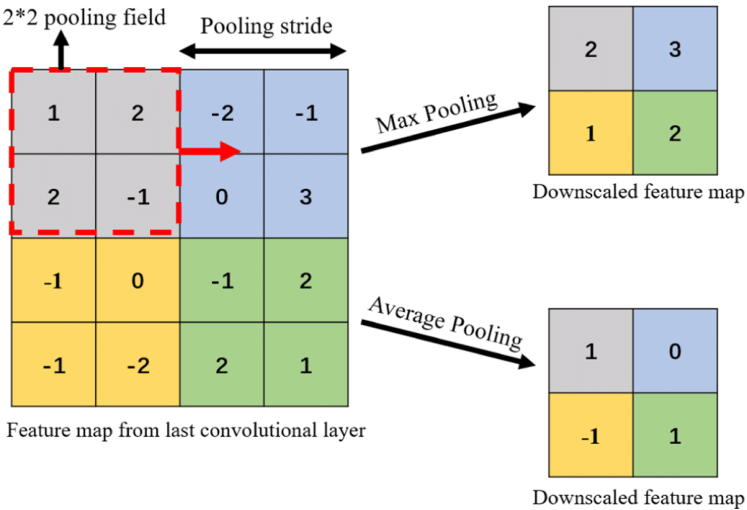
\includegraphics{Examples-for-max-and-average-pooling-layer.png}
\caption{Example of max and average pooling on output of previous convolutional layer \cite{pooling_diag}}
\end{figure}
\end{center}
\subsection{Fully Connected Layer}
The final layer or layers in a CNN is the fully connected layer. These fully connected 
layers have each input connected to each output by a learnable rate. The final fully 
connected layer typically has the same number of output nodes as the number of classes
\cite{Yamashita2018}. This final output layer then includes an activation function 
which is typically different than the output function in the convolutional layers.
This output function is set dependant on the task the CNN model is trying to achieve.
In the case of the image classification problem a softmax activation function is 
typically used \cite{REN202351} since it can be used to determine what the image is most likely to contain.
The softmax function is defined as follows;

\begin{equation}
   \sigma(\vec{z})_i = \dfrac{e^{z_i}}{\sum_{j=1}^{K}e^{z_j}}
\end{equation}
where $\sigma$ is the softmax, $\vec{z}$ is the input vector, $e^{z_i}$ is the standard 
exponential function for input vector, $K$ is the number of classes and $e^{z_j}$ is the 
standard exponential function for output vector. The output vector generates a set of 
probabilites for each class in $K$ with the max being selected as the final classification 
of the image.
\subsection{Training}
Training the CNN is done through a method known as backpropogation. Backpropogation dates 
back to the 1960's and was popularised in a paper published in 1986 \cite{Rumelhart1986}.
Backpropogation is an iterative algorithm that aims to minimise the cost function through 
two passes of the CNN model. The forward pass operates as it would during the testing phase 
with raw inputs being provided to the input layer of the CNN. Then the data traverses the 
network and the final output is returned. This output is compared to the actual values 
in the training data and an error value is determined. A common method of calculating the 
error is the mean squared error (MSE) which is defined as;
\begin{equation}
   MSE = \dfrac{1}{n}\sum_{i=1}^{n}(Y_i - \hat{Y}_i)^2
\end{equation}
where n is the number of observations, $Y$ is the observed values and $\hat{Y}$ is the 
predicted values.

Once this MSE has been calculated the backwards pass takes this calculated error and 
propogates it back through the network. The backwards pass utilises a gradient descent 
method to determine the gradient for each weight and bias in the network layers and 
is used to inform the magnitude of change that can be applied to minimise the error in 
the next forward pass. By utilising the chain rule, calculating this change of parameters 
with the goal of minimising the error can be done efficiently. This two pass process is 
done a predefined number of times, often called the epoch, with the final weights and 
biases for each layer being the values used in the model for the testing phase. Determining 
an optimal value for this epoch will form the basis of investigation through this report 
since a balance must be struck between accuracy improvements and training time required.
Another concern for the CNN model is the possibility of overfitting and underfitting. This 
is where the model contains to many layers and learns the optimal values for the training 
set. This results in high accuracy when training however could result in underperformance 
on new data during testing. If this occurs it can be a sign that there are to many 
convolutional layers in the CNN and improved performance may be observed with a 
simpler network. Since this report uses pre designed networks the risk of this is minimal 
however it needs to be monitored when investigating the impact of parameter changes.
\section{Pytorch}
Although it is possible to build a CNN from scratch, open source tools have allowed for 
rapid development and implementation of these models. Pytorch is one of these tools which 
is available in the Python programming language. Pytorch enables rapid prototyping of 
different models through its publishing of base implementations on a large number of 
common machine learning models. For the models investigated in this report, a base Pytorch
implementation was available for each of them. Thes models will be described in section 4 
of this report. Pytorch exposes low level api calls that allow the user to modify the models 
which greatly aids in the types of investigation and experimentation that are possible.
Pytorch can be used for model training and testing and provides robust functionality for 
the end to end process of defining and then using a given machine learning model.
Pytorch has native support for running this models on GPU's through its Cuda integration.
Cuda is a parallel computing platform and programming model developed by NVIDIA \cite{Oh_2022}
that allows developers to copy data to supported graphics cards and utilise the highly 
parallel architecture inherent to GPU's to increase training time greatly. Since the training 
process involves large numbers of operations to be done on matrices, this work can be 
parallelised effectively for massive performance gains.

\section{Data}
As mentioned in the introduction, the dataset used for this report was the CIFAR-10 image 
dataset \cite{cifar-10}. The dataset is comprised of 60,000 32x32 colour images that contain 
a single entity of one of ten classes. These classes are airplane, automobile, bird, cat, deer,
 dog, frog, horse, ship and truck. This dataset is split into a training and a testing 
set with 50,000 of the images being used for training and the remaining 10,000 being used 
for testing

\begin{center}
   \begin{figure}[H]
   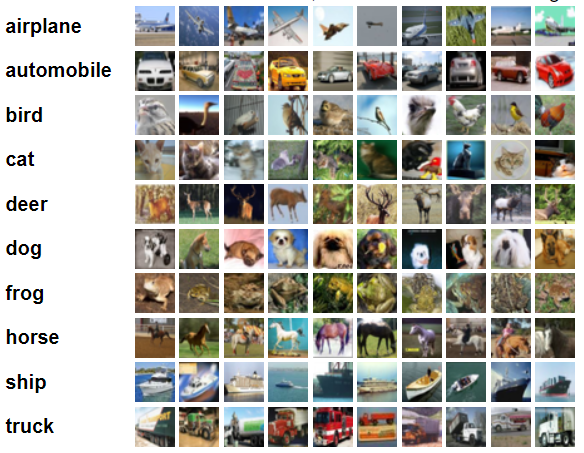
\includegraphics[scale=0.7]{cifar10.PNG}
   \caption{Examples of each class in the CIFAR-10 image dataset }
   \end{figure}
\end{center}

\section{Models}
Due to the maturity of CNN's and their application to the image classification problem,
a large number of models have been developed specifically for this application. Implementing 
a subset of these models will form the basis of the investigation on how modifying 
training parameters and training epochs can influence overall performance. The base implementation 
available in Pytorch will be used. 
\subsection{VGG-16}
VGG-16 contains three fully connected layers and 13 convolutional layers \cite{LINKON2021100582}.
It also contains five pooling layers that are placed consistently throughout the network.
There is a pooling layer after the first two convolutional layers and the third and fourth 
convolutional layer. Then there is a pooling layer after each set of three convolutional 
layers for the rest of the network. This is then followed by the three fully connected 
layers which provide the final output for the model. This architecture results in 16 
layers with learnable parameters.
\subsection{VGG-19}
VGG-19 is extremely similar to VGG-16 however an additional convolutional layer is added 
in the last three blocks. This results in an architecture of two convolutional layers, one 
pooling layer repeated twice. Then four convolutional layers, one pooling layer repeated 
three times. Then finally the three fully connected layers at the end of the network. 
VGG-19 has three additional layers with learnable parameters.

\subsection{ResNet-18}
The ResNet architecture differs from traditional neural networks. 
The ResNet-18 model contains a single convolutional layer initially then two pooling 
layers and eighteen convolutional layers between the pooling layers before a single 
fully connected layer. Traditionally when the network depth increases, accuracy gets 
saturated \cite{https://doi.org/10.48550/arxiv.1512.03385}. The ResNet architecture aims 
to address this performance degredation by introducing a deep residual learning framework.
This is achieved by implementing a residual block which contains a set of convolutional 
layers and a skip connection.Instead of learning a 
mapping, $H(x)$, to be fit by the stacked layers, the block learns $F(x) = H(x) - x$ or 
$H(x) = F(x) + x$ where x is the input to the to the first layer in the set. The output of 
the residual block is;
\begin{equation}
   Output = F(x,weights) +x
\end{equation}
where $F(x,weights)$ is the learned residual. The skip connections perform identitymapping, and their 
outputs are added to the output of the stacked layer \cite{https://doi.org/10.48550/arxiv.1512.03385}.
This allows the backpropogation process to effectively "skip" layers by focussing on the 
learned residual.
\subsection{ResNet-34}
The ResNet-34 model is functionally the same as the ResNet-18 model however instead of 
having eighteen convolutional layers between the pooling layers there are thirty four.
\subsection{ResNet-50}
As the ResNet architecture increases the number of convolutional layers a more efficient 
"bottleneck" design is used for the residual block. Each block is made of a 1x1,3x3 and 1x1 
covolution \cite{https://doi.org/10.48550/arxiv.1512.03385}. The 1x1 blocks are made for dimensionality reduction and expansion to the original 
dimensions. The 3x3 block is for feature extraction as normal. The skip connections are 
added between the start and end of each of these blocks. The ResNet-50 model replaces 
each two layer block present in the ResNet-34 netowkr with the bottleneck design resulting 
in a fifty layer network.
\section{Method}
CNN's have a number of parameters that can be set to alter the models final output and 
corresponding performance. An investigation into a subset of these was conducted and 
the results discussed. The key parameters shared across the investigated models were
backpropogation epoch, learning rate and batch size. For all the models a baseline 
implementation was built and its performance quantified. The metrics used to evaluate 
performance was accuracy, precision, recall and the F1 score. These were calculated through the confusion 
matrix generated after running the test dataset through the model. In a multi class 
classification problem such as image classification, the generation of a confusion 
matrix becomes more complex than the binary classification space. The confusion matrix 
is an $nxn$ matrix with $n$ being the number of classes. Each entity type has a row and 
column and the metrics are 
calculated on a per entity type basis. To retrieve the overall values for the metrics 
the mean of each is calculated and returned as the final result.

Accuracy calculates what proportion of the classifications were correct and is defined as;
\begin{equation}
   Accuracy = \dfrac{P_{correct}}{P_{correct} + P_{incorrect}}
\end{equation}
where $P$ is the prediction made.

Precision is a measure of the correctness of positive predictions which in the multi class 
image classification problem can answer the question out of all the predictions made, what 
proportion were actually the predicted class? This can be defined as;
\begin{equation}
   Precision = \dfrac{1}{n}\sum_{i=0}^{n}\dfrac{M_{ii}}{\sum_{j}^{}M_{ji}}
\end{equation}
Where $M$ is the confusion matrix, $n$ is the number of classes

Recall is a measure of the proportion of correct predictions for a class out of all the cases where 
that specific class. It is a measure of the number of times the model correctly identifies 
a given class from all the actual instances of that class in a dataset. This can be defined as;
\begin{equation}
   Recall = \dfrac{1}{n}\sum_{i=0}^{n}\dfrac{M_{ii}}{\sum_{j}^{}M_{ij}}
\end{equation}

The F1 score is the harmonic mean of precision and recall and is defined as;
\begin{equation}
   F1 Score = \dfrac{2*Precision*Recall}{Precision+Recall}
\end{equation}

Given the time it takes to train a new model on each parameter change, the impacts to performance 
will be performed on one of each type of model. For this investigation the VGG-16 and ResNet-18
models were investigated since they are the models of each type with the smallest number 
of convolutional layers and should provide representative performance changes as a result 
of the hyper parameter investigations.

To investigate the effect different epochs have on model performance during the backpropogation
process a set of values will be investigated. The baseline epoch used for all the models 
is 10 and the values 1,3,5,7,10,15,20,40 and 80 will be tested. Similarly the learning rate 
will be tested with a set of value with a baseline of 0.001. The values tested will be, 0.1,
0.01,0.001 and 0.0001. Finally the batch size will be investigated with a baseline of 32 
and the values investigated will be 8,16,32 and 64.

As the pretrained models are being used and they have been trained more effectively 
than the hardware available to this project, freezing of the model parameters will be done.
This involves not updating the parameters except in the final fully connected layer which 
needs to be done to only predict one of the ten classes in the CIFAR-10 dataset. This will 
greatly increase the speed of training and will allow the leveraging of the well trained 
models capabilities. It can also reduce the risk of overfitting as if the model was 
solely trained on the CIFAR data then it may learn features inherent to it reducing the models 
generalisation abilities. Loss will be caluclated through cross entropy loss, also known 
as log loss and for the multiclass classification can be defined as,
\begin{equation}
   Loss(\hat{y},y) = -\sum_{k}^{K}y^klog\hat{y}^k
\end{equation}
where $y^k$ is 0 or 1 indicating whether the class label $k$ is the correct classification \cite{Zafar_Tzanidou_Burton_Patel_Araujo}.

Finally the images will be preprocessed through resizing them to a 224x224 image which 
are the dimensions that the underlying models being used were trained on. Then
normalizing them using the mean and standard deviations of the images that the pretrained 
models were trained on. This will allow the model to be further trained on images that are similar 
in shape and scale to which they were initially trained on thus theoretically improving
model performance
\section {Results}
\subsection{Baseline}
As discussed in the method section, the first step of the investigation into the effects 
of modifying the hyper parameters a set of baseline results must be obtained. With epoch = 10,
learning rate = 0.001 and batch size = 32 Table  \ref{baselineresults} shows the gathered 
metrics.
\begin{table}[H]
\begin{center}
   \label{baselineresults}
   \begin{tabular}{||c c c c c||} 
    \hline
    Model & Accuracy & Precision & Recall& F1 Score \\  
    \hline\hline
    VGG16 & 0.870 & 0.875 & 0.870 & 0.872 \\ 
    \hline
    VGG19 & 0.882 & 0.885 & 0.882 & 0.883\\
    \hline
    ResNet18 & 0.903 & 0.904 & 0.903 & 0.902\\
    \hline
    ResNet34 & 0.907 & 0.910 & 0.908 & 0.908 \\
    \hline
    ResNet50 & 0.892 & 0.894 & 0.892 & 0.892 \\
    \hline
   \end{tabular}
   \caption{Baseline metrics for all investigated models}
\end{center}
\end{table}
It can be observed that the best performing model out of the VGG models is VGG19 with the 
highest values for all computed metrics. For the ResNet models, ResNet34 performed the best 
again with the highest metrics across the board.
\subsection{Epoch Investigation}
Determining an optimal or near optimal epoch value is important as it influences future 
hyper parameter investigations. Due to the training time required it is infeasible to 
test every combination of each hyper parameter as the number of models to be trained 
increases exponentially as the search space expands. As such each hyper parameter will 
be investigated in isolation. The impacts of this on the validity of the results will be 
discussed in the Discussion and Future Work sections of the report. The results of the 
epoch investigation are outlined in Table 2
\begin{table}[H]
   \begin{center}
      \label{vgg16epochinvestigation}
      \begin{tabular}{||c c c c c||} 
       \hline
       Epoch & Accuracy & Precision & Recall& F1 Score \\  
       \hline\hline
       1 & 0.842  & 0.852 & 0.842 & 0.843 \\ 
       \hline
       3 & 0.861  &  0.868& 0.861 & 0.862\\
       \hline
       5 & 0.864  &0.872 & 0.864 & 0.866\\
       \hline
       7 & 0.871 & 0.877 & 0.871 & 0.872 \\
       \hline
       10 & 0.870 & 0.875 & 0.870 & 0.872 \\
       \hline
       15 & 0.862 & 0.883 & 0.862 & 0.866 \\
       \hline
       20 & 0.874 & 0.880 & 0.874 & 0.875 \\
       \hline
       40 & 0.868 & 0.882 & 0.868 & 0.873 \\
       \hline
       80 & 0.860 & 0.884 & 0.861 & 0.867 \\
       \hline
      \end{tabular}
      \caption{Epoch results for VGG16}
   \end{center}
   \end{table}
Interestingly the accuracy values are almost identical to the recall results. This occurs 
when the dataset is balanced, has a roughly even number of each class. This will be investigated 
further in the Discussion section. These results are plotted in the below image;
\begin{center}
\begin{figure}[H]
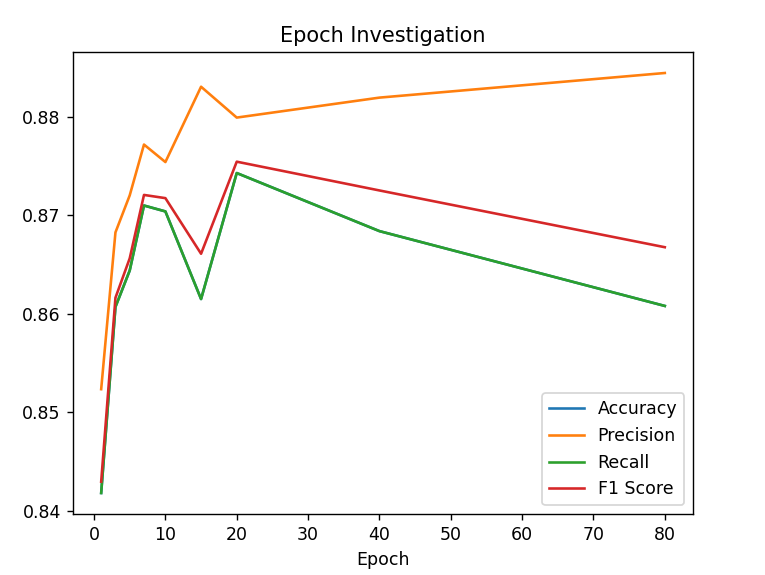
\includegraphics[scale=0.6]{epochinvestigation.PNG}
\caption{Plotted output from Table 2}
\end{figure}
\end{center}
Plotting the same set of epochs for the ResNet18 model yields the plot shown in Figure 4.
\begin{center}
   \begin{figure}[H]
   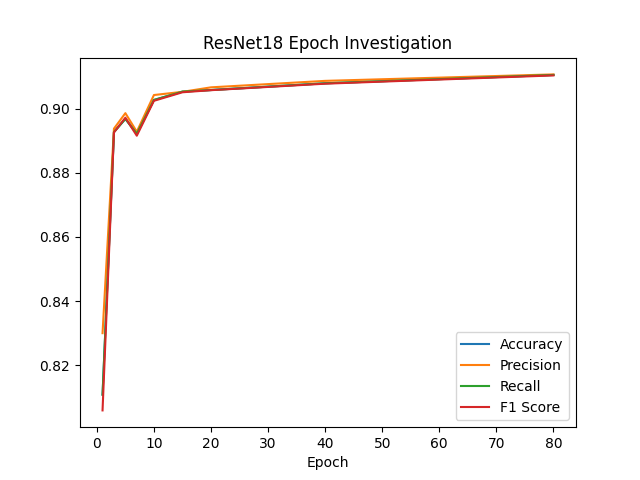
\includegraphics[scale=0.6]{resnet18epoch.png}
   \caption{ResNet18 epoch investigation results}
   \end{figure}
   \end{center}
Unlike the VGG16 model, the metrics continue to increase as the number of epochs investigated 
increases. The vlues investigated values clearly indicate the optimal value has not been found 
however the amount of performance increase doesnt appear to change much for epochs greater 
than 20. Balancing the time taken to train each new model with epochs greater 
than the upper bound used, 80, and the corresponding increase to performance, an epoch 
value of 20 has been found to be a suitable value. 

\subsection{Learning Rate Investigation}
When investigating the impact learning rate has on the overall model performance, the results 
from the epoch investigation were used as a baseline. That is the number of epochs used was
20 as that was found to have the best performance. As discussed in the Method section, 
the investigated values were 0.1,0.01,0.001,0.0001,0.00001 and 0.000001. The metrics were found 
and are displayed in Table 3 and were plotted in figure 5.
\begin{table}[H]
   \begin{center}
      \label{vgg16lrinvestigation}
      \begin{tabular}{||c c c c c||} 
       \hline
       LR & Accuracy & Precision & Recall& F1 Score \\  
       \hline\hline
       0.1 & 0.100  & 0.110 & 0.100 &0.018 \\ 
       \hline
       0.01 & 0.100  &  0.110& 0.100 &0.019\\
       \hline
       0.001 & 0.874  &0.880 & 0.874 & 0.875\\
       \hline
       0.0001 & 0.887 & 0.889 & 0.887 & 0.887 \\
       \hline
       0.00001 & 0.895 & 0.896 & 0.895 & 0.895 \\
       \hline
       0.000001 & 0.878 & 0.878 & 0.878 & 0.877 \\
       \hline
       \hline
      \end{tabular}
      \caption{Learning rate results for VGG16}
   \end{center}
   \end{table}
   \begin{center}
      \begin{figure}[H]
      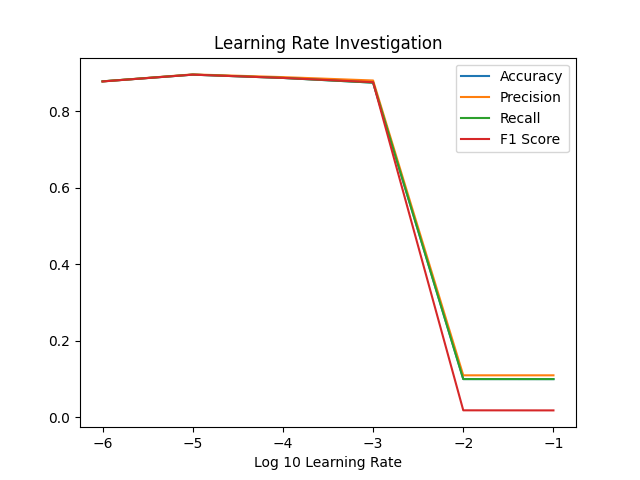
\includegraphics[scale=0.6]{lr_investigation.png}
      \caption{Plotted output from Table 3}
\end{figure}
\end{center}
\subsection{Batch Size Investigation}
As mentioned in the method section of the report the investigation into the batch size's 
impact of model performance was done using batch sizes of 8, 16, 32 and 64. The 
theoretical impact of altering the batch size will be discussed in the Discussion section 
of this report. For this investigation the VGG16 model was once again used with a learning 
rate of 0.00001 and 20 epochs. Setting this learning rate and epoch statically may not 
be an optimal solution however this will also be discussed later.
\begin{center}
   \begin{figure}[H]
   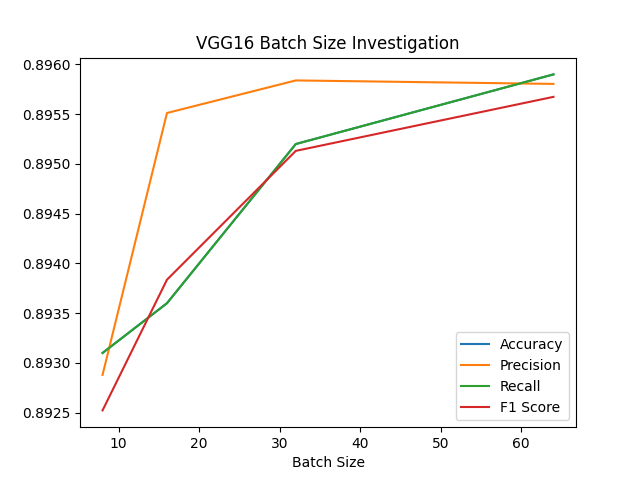
\includegraphics[scale=0.6]{batch_size_investigation.png}
   \caption{Batch size investigation results}
   \end{figure}
   \end{center}
From figure 6 it can be observed that as the batch size increases, the models performance 
trends upwards.

\section{Discussion}
CNN's expose a number of parameters that can be modified to impact overall performance.
Throughout this report a subset of these have been chosen and investigated to measure
each of their impacts. The epoch value determines the number of iterations of
backpropogation that occurs during the training process. Increasing the number of epochs 
allows the model more iterations for optimising the gradient to the training dataset.
More opportunities for optimising feature extraction and detection within the model 
are provided however a balance needs to be struck to avoid overfitting. Overfitting 
is where the model becomes to optimised at maximising performance on the training 
data and reduces the performance when new data is presented to the model. The epoch 
investigation on the VGG16 model showed that model performance when measured by recall,
f1 score and accuracy peaked at an epoch value of 20. The precision metric continued 
increasing as the epoch value increases which implies that the models performance on 
its positive predictions continues to increase. That is the number of true positives 
compared with the total number of positive predictions continues to increase. This 
is paired with a decrease in the models recall which incorporates false negatives in 
its calculation and implies that the model is generating more false negatives as the 
epoch value increases. A different observation was made when the ResNet18 model was
investigated as the metrics continued to increase as the epoch value exceeded the upper 
bound tested, 80. This implies that the optimal value for the epoch was not found 
in this report and in the future work section this will be expanded on. The impact 
of selecting the right epoch is drastic with the performance difference between an 
epoch of 1 and the optimal value for the VGG16 model being approximately 3.2\% 
and with the ResNet18 model the difference being almost 10\%.
\\
\\
The learning rate controls the rate at which the parameters at each layer are updated 
throughout the training process. A higher learning rate results in a greater rate of change.
If the learning rate is set to high then the model will likely reach its optimal performance 
quicker however the optimal parameter values found may overshoot the models actual 
optimal values resulting in degraded performance. This is caused by the model 
"overshooting" the optimal values and the learning rate used not providing the granularity
required. This needs to be balanced against the number of epochs required for the 
corresponding learning rate to converge on the optimal parameter values. With a smaller 
learning rate the number of iterations will be increased. From the investigation 
conducted into how the learning rate impacts the models overall performance, if the 
clearly unsuitable values are ignored , 0.1 and 0.01, the optimal learning rate can yield 
another approximately 2\% performance increase. 
\\
\\
The batch size investigation suggested that as the batch size increased, the model 
performance also increases. By increasing the batch size the backpropogation process 
utilises more of the training data resulting in smoother gradient updating. It does 
come with the risk of overfitting the data as this larger rate of change of the parameters 
runs the risk of getting stuck at local minima or maxima values resulting in not returning 
the optimal values. The size of the batches used also relies on the learning rate being 
appropriately tuned. For the investigation conducted in this report the learning rate 
was statically set. A smaller batch size relies on a smaller learning rate otherwise 
there is a risk of missing the optimal solution. On the other hand, a larger batch 
size can tolerate a larger learning rate however it still needs to be effectively tuned 
to avoid poor convergence and generalisation.
\\
\\
A potential issue that could have impacted the results is that for this investigation, 
the base models used before training was the pretrained version published by Pytorch.
Since the cifar10 dataset is a commonly used dataset, it is safe to assume that the 
dataset was used in the pretrained model. Performance was found to be significantly 
better after training the models on the cifar10 dataset. Each of the models investigated 
used the pretrained versions therefore providing a consistent base for the investigations 
conducted. Future work to repeat these investigations without the pretrained base will 
be expanded in the future work section. 
\section{Future Work}
For future work on this project, further investigations will be done on finding the optimal 
epoch value for the ResNet18 models. As mentioned in the discussion, for the epochs that were
tested the models performance was still increasing. This implies that the optimal epoch 
has not been found. Continuing to train ResNet18 models with increasing epochs to identify 
the inflection point will be done. Throughout this report the VGG16 and ResNet18 models 
were used for the various hyper parameter investigations, assumptions have been made 
that the findings for these models will be consistent with the different forms of the 
models. An investigation into this assumption will be completed by training each 
form of the models on the found optimal values for the parameters. Then determining 
that the performance gains found are replicated in the other models.

Only a subset of available CNN's were investigated in this report. Expanding this subset 
will be investigated in future work. Some of the other models to investigate are the 
AlexNet and GoogLeNet architectures. Re-running the investigations on the 
base versions of the models made available in Pytorch will be conducted. Determining 
the impact that the pretrained model has on model performance for the cifar10 dataset 
will be identified. Determining if model overfitting has tainted the results will need 
to be found and model performance using the found optimal values will be investigated.
It is expected that performance will be reduced as the pretrained versions of the models 
have undergone a robust training process on a huge dataset. This report has ignored 
the time portion of model training, however this is a key consideration when determining 
optimal model parameters. Given an infinite time horizon the absolute optimal values 
can be determined. Future work will include investigating the impact that modifying
parameters has on the overall time taken for training the model.
%-------------------------------------------------------------------------
\small
\bibliographystyle{ieee_fullname}
\bibliography{egbib}

\section{Appendix}
\end{document}
